\shorthandoff{"}
\chapter{Forschungsergebnisse}
\label{ch:ergebnisse}

\section{Fähigkeiten und Präferenzen der Mitarbeiter}
\label{ch:ergebnisse:analyse}
An der Umfrage unter den Projektmitarbeitern haben N=23 Personen im Fachbereich \acl{JES} der EXXETA AG teilgenommen. Es ist festzustellen, dass diese Angestellten insgesamt 643 Kompetenzbewertungen im Intranet des Unternehmens abgegeben haben. Das entspricht ca. 30 vergebenen Beurteilungen pro Person. Die Bewertungen verteilen sich auf insgesamt 212 der \anzFaehigkeiten unterschiedlichen im Intranet gespeicherten Fähigkeiten. Java ist mit 16 Beurteilungen die meist bewertete Kompetenz. Abbildung \ref{fig:diskussion:analyse:abb1} zeigt die bewerteten Fähigkeiten sortiert nach Anzahl an Beurteilungen. Dabei ist der der in Kapitel \ref{ch:empfehlungssysteme:cf:speicherbasiert} vorgestellte lange (Ratten-)Schwanz sehr gut erkennbar.

\begin{figure}[h]
	\centering
	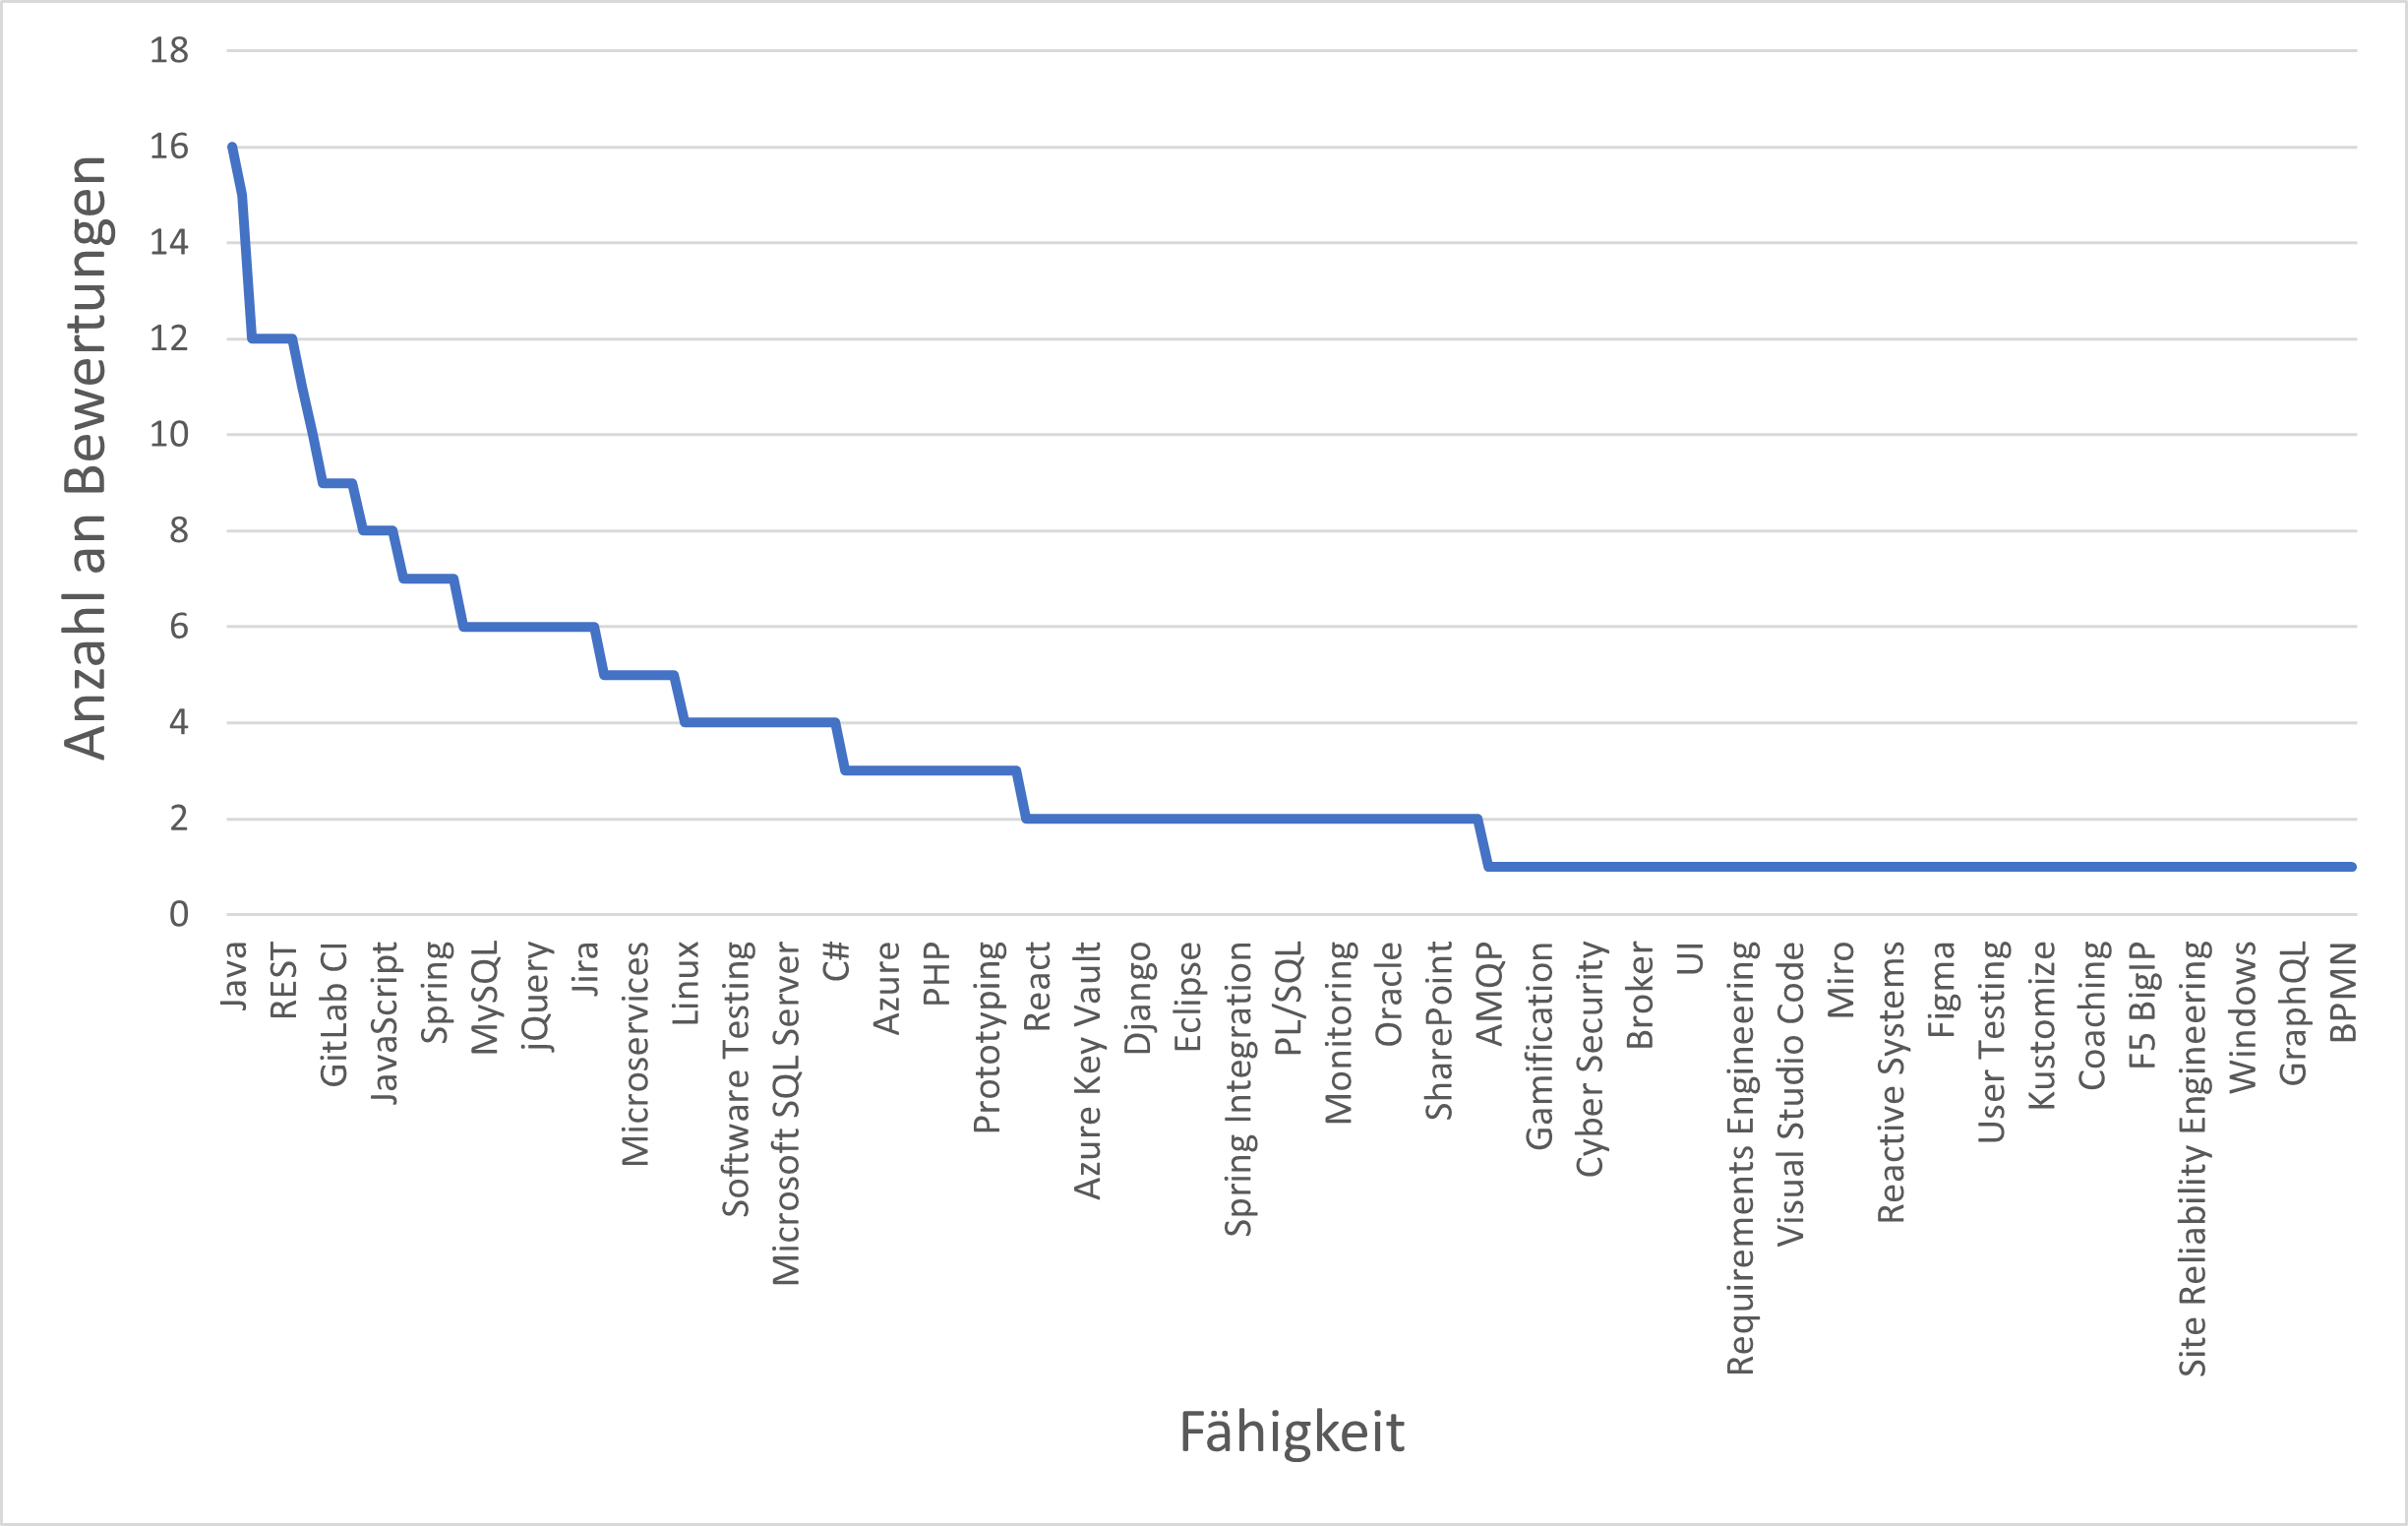
\includegraphics[width=1\textwidth]{gfx/long-tail-intranet.png}
	\caption{Langer (Ratten-)Schwanz bei den Fähigkeitsbewertungen im EXXETA-Intranet}
	\label{fig:ergebnisse:analyse:abb1}
\end{figure}

In Abbildung \ref{fig:diskussion:analyse:abb1} ist bezüglich des langen (Ratten-)Schwanzes zu erkennen, dass neun bzw. etwa 4.25 Prozent aller Fähigkeiten über zehn oder mehr Bewertungen verfügen. Dagegen haben 151 bzw. etwa 71.23 Prozent aller Kompetenzen drei oder weniger Beurteilungen.

Darüber hinaus ist für vier bzw. etwa 17.39 Prozent der Mitarbeiter ein Kaltstart zu erwarten. Diese haben bislang im Intranet keine einzige Fähigkeit bewertet. Der Grund hierfür ist


\newpage




Kaltstart: 4 Nutzer (17,39 Prozent) haben gar keine Fähigkeiten angegeben / Es sind immer mind. 19 andere Personen auf einem Skill verbunden

Projekt A: unilateral/bilateral\\
Projekt B: bilateral/unilateral\\
Projekt C: bilateral/unilateral\\
Projekt D: unilateral/bilateral\\
Projekt E: unilateral/bilateral

\shorthandon{"}
